\documentclass[12pt]{article}
\usepackage[utf8]{inputenc}
\usepackage[T2A]{fontenc}
\usepackage[russian]{babel}
\usepackage{amsmath}
\usepackage{amssymb}
\usepackage{dsfont}
\usepackage[dvipsnames]{xcolor}
\usepackage{setspace}
\usepackage{multirow}
\usepackage[a4paper, outer=1.5cm, inner=1.5cm, top=1cm, bottom=1cm]{geometry}
\usepackage{graphicx}
\usepackage{skull}
\usepackage{wasysym}
\usepackage{float}
\graphicspath{{.images/}}
\usepackage{hyperref}
\hypersetup{colorlinks=true, linkcolor=blue, filecolor=magenta, urlcolor=cyan}
\usepackage[firstpage]{draftwatermark}
\SetWatermarkText{
    $\qquad\qquad\qquad\qquad\qquad$\parbox{7cm}{\begin{center}
    
\includegraphics[width = 0.08\textwidth]{lion-logo.png}\bigskip\\~\bigskip\\~\vspace{-24mm}\\~\end{center}}
}
\SetWatermarkAngle{0}
\SetWatermarkScale{1.5}
\usepackage{etoolbox}

\newtoggle{ifsolved}
\newtoggle{needhelp}
\newcounter{num}
\setcounter{num}{1}

\newcommand{\newnum}{\par\textbf{\textnumero\arabic{num}}\stepcounter{num}}
\newcommand{\sol}{\vspace{3mm}\par\textbf{Решение: }}
\newcommand{\ans}{\vspace{3mm}\par\textbf{Ответ: }}
\newcommand{\hint}{\vspace{3mm}\par\textbf{Подсказка: }}
\newcommand{\mode}[1]{
\ifstrequal{#1}{0}{\togglefalse{ifsolved}\togglefalse{needhelp}}{\ifstrequal{#1}{1}{\togglefalse{ifsolved}\toggletrue{needhelp}}{\ifstrequal{#1}{2}{\toggletrue{ifsolved}\togglefalse{needhelp}}{\toggletrue{ifsolved}\toggletrue{needhelp}}}}} %if 0 - if 1 - if 2 - else
%\newenvironment{problem}[8]{%#1, #2, #3
%\parbox{\linewidth}{\vspace{4mm}\ifstrequal{#4}{(лёгкая)}{\newnum\textbf{.}}{\newnum\textbf{*.} } \\ #5}
%\iftoggle{ifsolved}{\sol #6}{}
%\iftoggle{ifsolved}{\ans #7}{}
%\iftoggle{needhelp}{\hint #8}{}}

\newenvironment{problem}[8]{%#1, #2, #3
\parbox{\linewidth}{\vspace{5mm}\ifstrequal{#4}{(лёгкая)}{\newnum\textbf{.}}{\newnum\textbf{*.} } \\ #5}
\iftoggle{ifsolved}{\sol #6}{}

\iftoggle{ifsolved}{\parbox{\linewidth}{\ans #7}}{}
\iftoggle{needhelp}{\parbox{\linewidth}{\hint #8}}{}}

\newenvironment{mylist} %custom list
{ \begin{itemize}
    \setlength{\itemsep}{0pt}
    \setlength{\parskip}{0pt}
    \setlength{\parsep}{0pt}     }
{ \end{itemize}                  }

\newenvironment{homeass}[1]{\vspace*{-1.5cm}
\iftoggle{ifsolved}{
    \section*{\center{Решение домашнего задания к #1.}}
}{
    \section*{\center{\textcolor{Sepia}{Домашнее задание к #1}}}
} \vspace{7mm}\large}

\parindent=0pt
\pagestyle{empty}
%$\!$[\arabic{class}.\arabic{num}]
%\ifnumcomp{\value{counter}}{>}{1}{true}{false}
%\definecolor{Gray}{gray}{0.9}
%\definecolor{mypink}{RGB}{219, 48, 122}
%\newcolumntype{g}{>{\columncolor{Gray}}p{2.8cm}}

\begin{document}
\large
\mode{7}
%0 for problems without hints
%1 for problems + hints
%2 for problems + solutions + answers
%else: show all

{\centering\section*{СПИСОК ЗАДАЧ}}

{\centering\subsection*{\smallskip\\\textcolor{green}{\textbf{Полезные вещи, которые можно и нужно копипастить:}}}}

\subsection*{\textcolor{Emerald}{\textbf{Полезные шпаргалки по LaTeXу:}}}

\textbf{Пример вставки рисунка:}

\begin{minipage}{\linewidth}
    \begin{minipage}{0.54\linewidth}
    см. рисунок справа\\
    Текст к собственно пикче, примерно всегда это либо развёрнутое описание, либо большая часть решения задачи --- стремимся экономить пространство, если это можно сделать.
    \end{minipage}
    \hspace{0.05\linewidth}
    \begin{minipage}{0.4\linewidth}
    \begin{figure}[H] 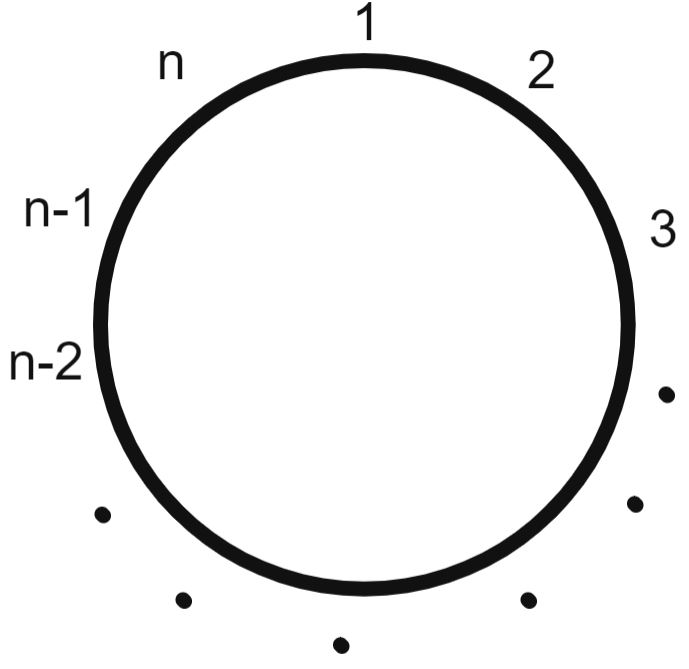
\includegraphics[width=\linewidth]{sol3} %тут поменять имя пикчи
    \end{figure}
    \end{minipage}
\end{minipage}

\textbf{Дефолтные математические знаки и символы:}\\
$\geqslant$,
$\leqslant$,
$a^{b}$,
$x_{i}$,
$\sqrt{a}$,
$\frac{a}{b}$,
$\displaystyle \frac{a}{b}$,
$\cdot$
$\;\Rightarrow\;$,
$\;\Leftrightarrow\;$,
$1{,}2$.
О промежутках:
$a\!b$,
$a\,b$,
$a\:b$,
$a\;b$,
$a\quad b$.

\textbf{Стандартные система и совокупность уравнений / неравенств:}\\
$\left\{
\begin{aligned}
f(x) &= 0 \\
g(x) &= 1
\end{aligned}\right.$

$\left[\begin{aligned}
&\left\{\begin{aligned}
f(x) &\geqslant a \\
g(x) &= b
\end{aligned}\right.\\
&\left\{\begin{aligned}
f(x) &< a \\
g(x) &= -b
\end{aligned}\right.
\end{aligned}\right.$

\subsection*{\textcolor{Emerald}{\textbf{Не математическое, но полезное:}}}
% комментарий в любом месте документа, который нигде не будет видно. Можно использовать для написания заметок-вопросов по задачам
\textbf{Пример таблицы:}

\begin{tabular}{|c|c|c|}
\hline
    $a$ & $b$ & текст
\\\hline
    $c$ & $d$ & мораль
\\\hline
\end{tabular}\\

\textbf{Отступы:} между\smallskip\\ строками\medskip\\ \textbf{Тире} --- это три дефиса.\\
\textbf{Списки:}
\begin{mylist}
\item [$\bullet$] это был пункт а
\item [2)] а это уже пункт номер 2 с изменённым заголовком
\end{mylist}

\subsection*{\textcolor{Emerald}{\textbf{Всё, неупомянутое выше (или если просто что-то не так):}}}
\begin{mylist}
\item [$\bullet$] Решение отдельных вопросов касательно ТеХа нужно искать в \href{https://www.mccme.ru/free-books/llang/newllang.pdf}{Львовском}.

\item [$\bullet$] Найти произвольный символ, который нужен, можно в \href{http://detexify.kirelabs.org/classify.html}{Detexify}.

\item [$\bullet$] Если возникли сомнения при решении, ответ практически ко всем задачам можно проверить с помощью \href{https://www.wolframalpha.com/}{WolframAlpha}.

\item [$\bullet$] Если в задаче нужно создать картинку, то лучше пока отложить эту задачу. Все графики планируется централизованно нарисовать (или перерисовать) в геогебре.

\item [\textcolor{brown}{\textbf{!!}}] Важно ставить \textcolor{red}{\textbf{$\spadesuit$}}
(или просто red) в тело задачи в случае серьёзных вопросов к решению и какой-то вопиющей лажи.

\item [\textcolor{brown}{\textbf{!!}}] Важно ставить \textcolor{olive}{\textbf{$\spadesuit$}}
(или просто olive) в тело задачи в случае не самого удачного текста и кривых отступов.
\end{mylist}

\subsection*{\textcolor{Violet}{\textbf{Комментарии:}}}% а также невидимые комментарии - так можно оставлять заметки-вопросы прямо в задаче, чтобы потом было понятно, в чём вопрос.
\begin{mylist}
\item [$\skull$] Переставлять задачи местами --- очень плохая идея.

\item [$\smiley$] При двойном клике по тексту pdf справа происходит автоматический переход к этому месту в латех-коде, а для обратного перехода можно нажать стрелку вправо (висит сверху между pdf и латех-кодом).

\item [$\smiley$] Если есть размышления, дописывать red/olive к задаче или не дописывать, то лучше всё-таки дописать.

\item [$\skull$] Самое плохое, что можно сделать --- написать в любое поле из трёх (НаписанноеРешение/ВерныйОтвет/Подсказка) только половину того, что надо, никак это не отметить, и потом пойти дальше.\\ Нужно в этот момент писать red/olive в случайном месте задачи, чтобы потом вычислить это с помощью Ctrl+F по всему документу (и это то, что потом будет делаться долго и тщательно)
\end{mylist}

\newpage
\setcounter{num}{1636}

\hypertarget{11.1}{{\centering\section*{\bigskip\\\textcolor{Blue}{\hyperlink{start2}{\textcolor{Blue}{11.1}} Комплексные числа.}\vspace{-5mm}}}}

\begin{problem}{Комплексные числа. Их свойства, арифметические операции.}{11.1.1}{11D}{(лёгкая)}
{Чему равно произведение чисел $a + bi$ и $c + di$?}
{НаписанноеРешение}
{ВерныйОтвет}{Подсказка}
\end{problem}

\begin{problem}{Комплексные числа. Их свойства, арифметические операции.}{11.1.1}{11D}{(лёгкая)}
{Чему равно число $\,\displaystyle \frac{a + bi}{c + di}$?}
{НаписанноеРешение}
{ВерныйОтвет}{Подсказка}
\end{problem}

\begin{problem}{Комплексные числа. Их свойства, арифметические операции.}{11.1.1}{11D}{(лёгкая)}
{Даны комплексные числа $z_1 = 2i$, $\,z_2 = 3 - 2i$, $\,z_3 = -1 + 3i$, $\,z_4 = 1 + 2i$.\\
Найти комплексные числа $z_1 z_2$, $\;z_1 + z_2 z_3$, $\;z_4^2 + (z_3 + z_2)z_1$, $\;z_1^4 + z_2^3 + z_3^2 + z_4$.}
{\begin{mylist}
    \item $z_1 z_2 = 2i \cdot (3 - 2i) = 6i - 4i^2 = 4 + 6i$.
    \item $z_1 + z_2 z_3 = 2i + (3 - 2i) \cdot (-1 + 3i) = 2i - 3 + 9i + 2i - 6i^2 = 3 + 13i$.
    \item $z_4^2 + (z_3 + z_2)z_1 = (1 + 2i)^2 + (-1 + 3i + 3 - 2i) \cdot 2i = 1 + 4i + 4i^2 + 4i + 2i^2 =$ $= -5 + 8i$.
    \item $z_1^4 + z_2^3 + z_3^2 + z_4 = (2i)^4 + (3 - 2i)^3 + (-1 + 3i)^2 + 1 + 2i = 16 + 27 - 54i - 36 + 8i + 1 - 6i - 9 + 1 + 2i = -50i$.
\end{mylist}\vspace{-2mm}}
{$\;z_1 z_2 = 4 + 6i$, \hfill $z_1 + z_2 z_3 = 3 + 13i$, \hfill $z_4^2 + (z_3 + z_2)z_1 = -5 + 8i$,\\ $z_1^4 + z_2^3 + z_3^2 + z_4 = -50i$.}{Использовать распределительный закон и определение $i$.}
\end{problem}

\begin{problem}{Комплексные числа. Их свойства, арифметические операции.}{11.1.1}{11D}{(лёгкая)}
{Решить уравнение в комплексных числах: $(1 + i) \cdot z = 3 - i$.}
{НаписанноеРешение}
{ВерныйОтвет}{Подсказка}
\end{problem}

\begin{problem}{Комплексные числа. Их свойства, арифметические операции.}{11.1.1}{11D}{(лёгкая)}
{Известно, что $z_1 = 1 + i$, а $z_2 = 2 - i$. Найти комплексное число $z = \frac{z_1}{z_2} - \frac{z_2}{z_1}$.}
{Для деления на комплексное число домножим дробь на сопряжённое знаменателю комплексное число. Тогда получаем: $\,\displaystyle z = \frac{z_1}{z_2} - \frac{z_2}{z_1} = \frac{1 + i}{2 - i} - \frac{2 - i}{1 + i} =$\smallskip\\ $\displaystyle =\frac{(1 + i)(2 + i)}{(2 - i)(2 + i)} - \frac{(2 - i)(1 - i)}{(1 + i)(1 - i)} = \frac{1 + 3i}{4 + 1} - \frac{1 - 3i}{1 + 1} = \frac{2 + 6i - 5 + 15i}{10} = -0{,}3 + 2{,}1i$.}
{Комплексное число $z = \frac{z_1}{z_2} - \frac{z_2}{z_1}\,$ равно $-0{,}3 + 2{,}1i$.}{Нужно домножить на сопряжённое знаменателю число, по аналогии с избавлением от иррациональности в знаменателе для обычных корней.}
\end{problem}

\begin{problem}{Комплексные числа. Их свойства, арифметические операции.}{11.1.1}{11D}{(лёгкая)}
{Операцией комплексного сопряжения называется переход от числа $z = a + bi$ к сопряжённому числу $\overline{z} = a - bi$. Доказать следующие свойства этой операции:\medskip\\
a) $\overline{\,\overline{z}\,} = z$. \hfill
b) $\overline{z_1 + z_2} = \overline{z_1} + \overline{z_2}$. \hfill
c) $\overline{z_1 z_2} = \overline{z_1} \cdot \overline{z_2}$.

}
{\vspace{-3mm}\begin{mylist}
    \item [a)] Пусть $z = a + bi$. Тогда $\overline{\,\overline{z}\,} = \overline{\,\overline{a + bi}\,} = \overline{a - bi} = a + bi = z$. Доказано.
    \item [b)] Пусть $z_1 = a + bi$, а $z_2 = c + di$. Тогда $\overline{z_1 + z_2} = \overline{a + bi + c + di} = $\\$ \overline{(a + c) + (b + d)i} = (a + c) - (b + d)i = a - bi + c - di = \overline{z_1} + \overline{z_2}$. Доказано.
    \item [c)] Пусть $z_1 = a + bi$, а $z_2 = c + di$. Тогда $\overline{z_1 z_2} = \overline{(a + bi)(c + di)} =$\\ $= \overline{(ac - bd) + (ad + bc)i} = (ac - bd) - (ad + bc)i$. С другой стороны, $\overline{z_1} \cdot \overline{z_2} = (a - bi)(c - di) = ac - adi - bci - bd = (ac - bd) - (ad + bc)i$. Доказано.
\end{mylist}\vspace{-2mm}}
{Смотри доказательства выше.}{Нужно использовать определение комплексного сопряжения.}
\end{problem}

\begin{problem}{Комплексные числа. Их свойства, арифметические операции.}{11.1.1}{11D}{(лёгкая)}
{Показать, что $z + \overline{z}\,$ и $z \cdot \overline{z}\,$ являются вещественными числами.}
{Пусть комплексное число $z$ равно $x + iy$, где $x$ и $y$~--- вещественные числа. Тогда $\overline{z} = x - iy \;\Rightarrow\; z + \overline{z} = x + iy + x - iy = 2x$.\\ $x$ является вещественным числом, следовательно, сумма числа и комплексно сопряжённого ему, вещественна. Теперь произведение: $z \cdot \overline{z} = (x + iy)(x - iy) = x^2 + y^2 = |z|^2$, поэтому произведение также является вещественным. Доказано.}
{Смотри рассуждения выше. $\,z \cdot \overline{z} = |z|^2$.}{Раскрыть скобки по распределительному закону.}
\end{problem}

\begin{problem}{Комплексные числа. Их свойства, арифметические операции.}{11.1.1}{11D}{*}
{Известно, что множество комплексных чисел $\mathbb{C}$ удовлетворяет трём свойствам:\\
1. $\mathbb{C}$ содержит некоторое число $i$, такое что $i^2 = -1$ (мнимую единицу).\\
2. $\mathbb{R} \subset \mathbb{C}$ (множество комплексных чисел содержит все действительные числа).\\
3. Операции сложения, вычитания, умножения и деления комплексных чисел имеют те же свойства, что и на множестве $\mathbb{R}$ (результат операции всегда определён, и верны сочетательный, переместительный, и распределительный законы).\\
Показать, что любое комплексное число имеет вид $a + bi$, где $a$ и $b$~--- вещественные числа.}
{НаписанноеРешение}
{ВерныйОтвет}{Подсказка}
\end{problem}

\begin{problem}{Комплексная плоскость.}{11.1.2}{11D}{(лёгкая)}
{Изобразить на координатной плоскости все комплексные числа, у которых:\\
a) Мнимая часть равна -2.\\
b) Действительная часть является нечетным однозначным натуральным числом.\\
с) Отношение действительной части к мнимой равно $-\frac12$.\\
d) Сумма квадратов действительной и мнимой частей равна 9.}
{a) Мнимая часть комплексного числа откладывается по вертикали, поэтому получается горизонтальная прямая $y = -2$.\smallskip\\
b) Вещественная часть откладывается по горизонтали, поэтому подходят 5 вертикальных прямых: $x = 1$, $x = 3$, $x = 5$, $x = 7$, и $x = 9$.\vspace{-2mm}\\\begin{minipage}{\linewidth}
    \begin{minipage}{0.44\linewidth}
    c) На обычной плоскости это будет эквивалентно уравнению $\frac{x}{y} = -\frac12$, а значит, получится прямая $y = -2x$ с выколотой точкой $O = (0; 0)$.\medskip\\
    d) Уравнение $x^2 + y^2 = 9$ задаёт окружность с центром в $O = (0; 0)$ и радиусом 3.\bigskip\\
    То, что в итоге получилось, изображено на рисунке справа.
    \end{minipage}
    \hspace{0.05\linewidth}
    \begin{minipage}{0.5\linewidth}\begin{figure}[H] 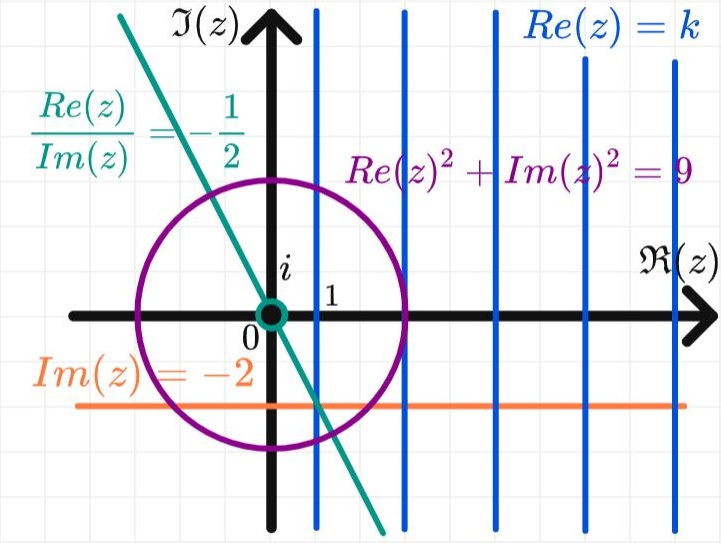
\includegraphics[width=\linewidth]{sol47}\end{figure}\end{minipage}
\end{minipage}}
{Смотри рисунок выше.}{В пункте с) следует быть осторожным с делением на 0.}
\end{problem}

\begin{problem}{Комплексная плоскость.}{11.1.2}{11D}{(лёгкая)}
{Известны два комплексных числа: $z_1 = 2 + i$, $\,z_2 = 1 - i$. Изобразить на координатной плоскости эти два числа, а также числа $-2z_2$, $\,z_1 + z_2$, $\,z_1 - z_2$, и $\,iz_1$.

}
{\vspace{-2mm}\\\begin{minipage}{\linewidth}
    \begin{minipage}{0.44\linewidth}
    Все полученные комплексные числа изображены на рисунке справа.\smallskip\\
    Видно, что если рассматривать комплексное число $a + bi$ как вектор $(a, b)$, то сложение и вычитание действуют как уже известные нам сложение и вычитание векторов, а умножение здесь~--- это некоторый поворот (на самом деле, комбинация поворота и растяжения). 
    \end{minipage}
    \hspace{0.05\linewidth}
    \begin{minipage}{0.5\linewidth}\begin{figure}[H] 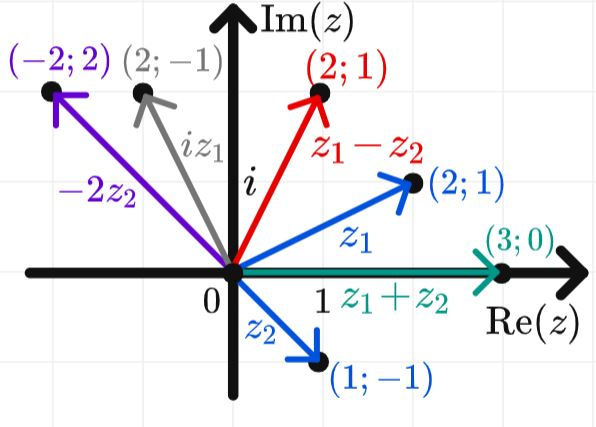
\includegraphics[width=\linewidth]{sol48}\end{figure}\end{minipage}
\end{minipage}}
{Смотри рисунок выше.}{$a + bi \;\Leftrightarrow\; (a, b)$.}
\end{problem}

\begin{problem}{Тригонометрическая форма записи комплексного числа.}{11.1.3}{11D}{(лёгкая)}
{Найти модуль числа $20 - 21i$.}
{По определению: $|z| = \sqrt{a^2 + b^2} = \sqrt{20^2 + (-21)^2} = \sqrt{400 + 441} = \sqrt{841} = 29$. Таким образом, модуль этого числа равен 29.}
{29.}{Использовать определение модуля комплексного числа.}
\end{problem}

\begin{problem}{Тригонометрическая форма записи комплексного числа.}{11.1.3}{11D}{(лёгкая)}
{Найти модуль числа $\,\displaystyle -\frac{6}{i}$.}
{Для того чтобы найти модуль комплексного числа, сначала приведём его к стандартному виду $z = a + bi$. Для этого домножим дробь на сопряжённое: $-\frac{6}{i} = -\frac{-6i}{-i^2} = 6i$. Модуль этого числа равен 6.}
{6.}{Для начала стоит привести комплексное число к стандартному виду.}
\end{problem}

\begin{problem}{Тригонометрическая форма записи комплексного числа.}{11.1.3}{11D}{(лёгкая)}
{Найти модуль числа $\,\displaystyle \frac{1 - i}{i}$.}
{НаписанноеРешение}
{ВерныйОтвет}{Подсказка}
\end{problem}

\begin{problem}{Тригонометрическая форма записи комплексного числа.}{11.1.3}{11D}{(лёгкая)}
{Проверить, что для действительных чисел $(b = 0)$ определение модуля в $\mathbb{C}$ совпадает с уже имеющимся.}
{Рассмотрим комплексное число $z = a + bi$. Его модуль равен $\sqrt{a^2 + b^2}$. При $b = 0$ получаем, что модуль комплексного числа равен $\sqrt{a^2 + 0^2} = \sqrt{a^2}$. \\ При этом, когда $b = 0$, получаем вещественное число $a + 0\cdot i = a$. Согласно определению модуля для вещественных чисел, получаем, что модуль равен $|a|$.\smallskip\\ Но $|a| \equiv \sqrt{a^2}$, поэтому новое определение модуля для комплексных чисел согласовано со старым (и о том, и о другом можно думать, как о длине отрезка, но один лежит на прямой $\mathbb{R}$, а другой~--- на декартовой плоскости $\mathbb{R}^2$).}
{Смотри рассуждения выше (оба модуля можно рассматривать как длины одинаковых отрезков).}{Сравни, что получится, если взять модуль по определению для\\ комплексного числа, и если взять его для вещественного числа $a$.}
\end{problem}

\begin{problem}{Тригонометрическая форма записи комплексного числа.}{11.1.3}{11D}{*}
{Пользуясь только определением модуля и свойствами умножения, доказать\\ теорему: $|z_1 \cdot z_2| = |z_1| \cdot |z_2|$ (модуль произведения равен произведению модулей).}
{Пусть $z_1 = a + bi$, а $z_2 = c + di$. Тогда $z_1 \cdot z_2 = (ac - bd) + (ad + bc)i$.\smallskip\\
$|z_1| \cdot |z_2| = \sqrt{a^2 + b^2} \cdot \sqrt{c^2 + d^2} = \sqrt{a^2c^2 + a^2d^2 + b^2c^2 + b^2d^2}$.\\
$|z_1 \cdot z_2| = \sqrt{(ac - bd)^2 + (ad + bc)^2} = \sqrt{a^2c^2 - 2abcd + b^2d^2 + a^2d^2 + 2abcd + b^2c^2}$.\smallskip\\
Видно, что в итоге $2abcd$ под корнем сокращаются друг с другом, и выражения получаются тождественно равными. Следовательно, $|z_1| \cdot |z_2| = |z_1 \cdot z_2|$.\smallskip\\
Теорема доказана: при умножении комплексных чисел их модули перемножаются.}
{Смотри рассуждение выше.}{Здесь срабатывает проверка равенства <<в лоб>>.}
\end{problem}

\begin{problem}{Тригонометрическая форма записи комплексного числа.}{11.1.3}{11D}{(лёгкая)}
{Аргументом ненулевого комплексного числа $z$ называют вещественное число\\ $\varphi \in (-\pi; \pi]$ такое, что $z = |z|(\cos\varphi + i\sin\varphi)$. Найти аргумент числа:\medskip\\
a) $2i$. \hfill
b) $-i$. \hfill
c) $-5$. \hfill
d) $3 - 3i$. \hfill
e) $1 + \sqrt{3}i$.}
{\vspace{-3mm}\begin{mylist}
    \item [a)] $2i = 2 \cdot (\cos\frac{\pi}{2} + i \cdot \sin\frac{\pi}{2})$. Поэтому в данном случае аргумент равен $\frac{\pi}{2}$.
    \item [b)] $-i = 1 \cdot \left(\cos\left(-\frac{\pi}{2}\right) + i \cdot \sin\left(-\frac{\pi}{2}\right)\!\right)$. В этом случае аргумент будет равен $-\frac{\pi}{2}$.
    \item [c)] $-5 = -5 \cdot (\cos\pi + i \cdot \sin\pi)$. Поэтому в данном случае аргумент равен $\pi$.
    \item [d)] $3 - 3i = 3\sqrt{2} \cdot \left(\cos\left(-\frac{\pi}{4}\right) + i \cdot \sin\left(-\frac{\pi}{4}\right)\!\right)$. Итого, аргумент равен $-\frac{\pi}{4}$.
    \item [e)] $1 + \sqrt{3}i = 2 \cdot \left(\cos\left(\frac{\pi}{3}\right) + i \cdot \sin\left(\frac{\pi}{3}\right)\!\right)$. Следовательно, аргумент равен $\frac{\pi}{3}$.
\end{mylist}\vspace{-2mm}}
{$\;\text{arg}(2i) = \frac{\pi}{2}$,\hfill $\text{arg}(-i) = -\frac{\pi}{2}$,\hfill $\text{arg}(-5) = \pi$,\hfill $\text{arg}(3 - 3i) = -\frac{\pi}{4}$,\\ $\text{arg}(1 + \sqrt{3} i) = \frac{\pi}{3}$.}{Угадывание углов в уме~--- не самая простая задача.\\ Для решения может быть проще нарисовать все точки на плоскости.}
\end{problem}

\begin{problem}{Тригонометрическая форма записи комплексного числа.}{11.1.3}{11D}{(лёгкая)}
{Изобразить на координатной плоскости все комплексные числа, у которых:\\
a1) модуль равен 3. $\qquad\quad\;\,$ a2) модуль равен 4. $\qquad\qquad\!$ a3) модуль равен 0.\\
b1) аргумент равен $\frac{2\pi}{3}$. \hfill b2) аргумент равен $-\frac{\pi}{5}$. \hfill b3) аргумент равен $\frac{3\pi}{4}$.}
{Комплексные числа с фиксированным аргументом $\varphi$ представляют собой открытый луч, выходящий из начала координат под углом $\varphi$ (для $z = 0$ аргумент не определён). \\ Комплексные числа $z = x + iy$ с некоторым фиксированным модулем $a$ удовлетворяют уравнению $x^2 + y^2 = a^2$, то есть лежат на окружности радиуса $a$.
\vspace{-2mm}\\\begin{minipage}{\linewidth}
    \begin{minipage}{0.58\linewidth}
    Поэтому получается следующая картина:\\ смотри рисунок справа.\medskip\\
    Видно, что модуль и аргумент однозначно определяют число, то есть вместо координат $(x, y)$ можно рассматривать координаты $(r, \varphi)$.\smallskip\\ Эта координатная система называется \textit{полярной системой координат} и может быть использована вместо декартовой (разумеется, особенно удобно её использовать, когда нужно рассмотреть окружности, эллипсы, или спирали).
    \end{minipage}
    \hspace{0.03\linewidth}
    \begin{minipage}{0.37\linewidth}\begin{figure}[H] 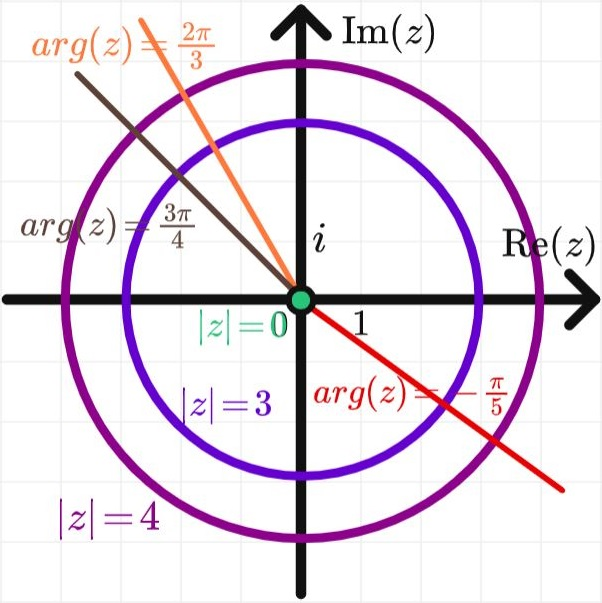
\includegraphics[width=\linewidth]{sol49}\end{figure}\end{minipage}
\end{minipage}}
{Смотри рисунок выше.}{Рисунок состоит из окружностей и открытых лучей.}
\end{problem}

\begin{problem}{Формула Муавра. Возведение комплексного числа в степень.
}{11.1.4}{11D}{(лёгкая)}
{Пусть $z_1 = |z_1|(\cos\alpha + i\sin\alpha)$, а $z_2 = |z_2|(\cos\beta + i\sin\beta)$.\\ Показать, что при произведении $z_1$ и $z_2$ их аргументы складываются по модулю $2\pi$, то есть что $\,z_1 \cdot z_2 = |z_1| \cdot |z_2|(\cos(\alpha + \beta) + i\sin(\alpha + \beta))$.}
{Используем распределительный закон: $z_1 \cdot z_2 = |z_1|(\cos\alpha + i\sin\alpha) \cdot |z_2|(\cos\beta + i\sin\beta) = |z_1||z_2|(\cos\alpha\cos\beta - \sin\alpha\sin\beta + i\sin\alpha\cos\beta + i\cos\alpha\sin\beta)$.\\ Можно заметить, что вещественная часть у полученного комплексного числа в точности равна $\cos(\alpha + \beta)$, а мнимая часть~--- в точности $\sin(\alpha + \beta)$. Поэтому $z_1 \cdot z_2 = |z_1| \cdot |z_2|(\cos(\alpha + \beta) + i\sin(\alpha + \beta))$. Из-за периодичности синуса и косинуса угол, получаемый в качестве ответа, известен нам с точностью до $2\pi$~--- поэтому по факту аргументы равны по модулю $2\pi$, а наше требование что $\text{arg}(z)\in(-\pi; \pi]$~--- только выбор некоторого <<основного>>, главного значения: с тем же успехом мы могли положить в определении аргумента $\varphi \in [0; 2\pi)$.}
{$|z_1|(\cos\alpha + i\sin\alpha) \cdot |z_2|(\cos\beta + i\sin\beta) = |z_1| \cdot |z_2|(\cos(\alpha + \beta) + i\sin(\alpha + \beta))$.

}{Используй распределительный закон.}
\end{problem}

\begin{problem}{Формула Муавра. Возведение комплексного числа в степень.
}{11.1.4}{11D}{(лёгкая)}
{Вычислить $(\cos 15^{\circ} + i\sin 15^{\circ})^6$.}
{НаписанноеРешение}
{ВерныйОтвет}{Подсказка}
\end{problem}

\begin{problem}{Формула Муавра. Возведение комплексного числа в степень.
}{11.1.4}{11D}{(лёгкая)}
{Вычислить $(1 + i)^{13}$.}
{НаписанноеРешение}
{ВерныйОтвет}{Подсказка}
\end{problem}

\begin{problem}{Формула Муавра. Возведение комплексного числа в степень.
}{11.1.4}{11D}{(лёгкая)}
{Число $c = \frac{\sqrt{2}}{2} + \frac{\sqrt{2}}{2}i$. Изобразить на координатной плоскости числа $c$, $\,c^2$, $\,c^3$, $\,c^7$.\\
Найти их аргументы.}
{Несложно отметить, что $|c| = \sqrt{\left(\frac{\sqrt{2}}{2}\right)^{\!2} + \left(\frac{\sqrt{2}}{2}\right)^{\!2}} = 1$. \vspace{-2mm}\\\begin{minipage}{\linewidth}
    \begin{minipage}{0.58\linewidth}
    ~\vspace{1mm}\\
    Более того, $c = 1 \cdot (\cos \frac{\pi}{4} + i \sin \frac{\pi}{4})$, то есть оно находится на единичной окружности и прямой $y = x$. Но при умножении модули перемножаются, а аргументы складываются.\medskip\\ Следовательно, $c^2 = \cos \frac{2\pi}{4} + i \sin \frac{2\pi}{4} = i$.\smallskip\\ $c^3 = \cos \frac{3\pi}{4} + i \sin \frac{3\pi}{4} = -\frac{\sqrt{2}}{2} + \frac{\sqrt{2}}{2}i$.\smallskip\\
    $c^7 = \cos \frac{7\pi}{4} + i \sin \frac{7\pi}{4} = \cos \left(-\frac{\pi}{4}\right) + i \sin \left(-\frac{\pi}{4}\right) = \frac{\sqrt{2}}{2} - \frac{\sqrt{2}}{2}i$.\bigskip\\ Аргументы этих чисел равны $\frac{\pi}{4}$, $\frac{\pi}{2}$, $\frac{3\pi}{4}$, и $-\frac{\pi}{4}$.
    \end{minipage}
    \hspace{0.03\linewidth}
    \begin{minipage}{0.37\linewidth}\begin{figure}[H] 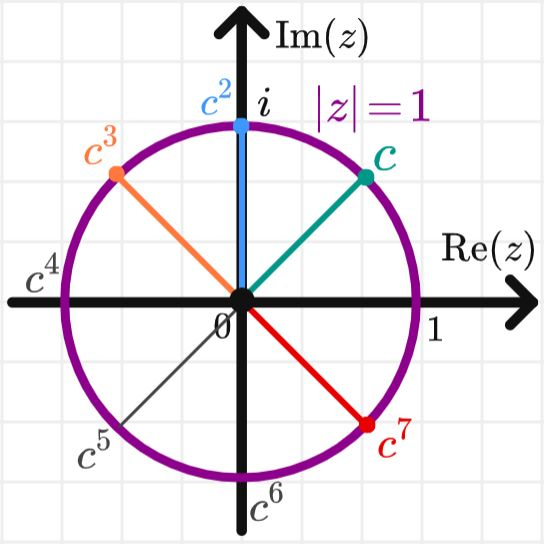
\includegraphics[width=\linewidth]{sol50}\end{figure}\end{minipage}
\end{minipage}}
{См. рисунок выше. $\arg(c) = \frac{\pi}{4}$, $\,\arg(c^2) = \frac{\pi}{2}$, $\,\arg(c^3) = \frac{3\pi}{4}$, $\,\arg(c^7) = -\frac{\pi}{4}$.}{Лучше всего записать число $c$ в тригонометрической форме.}
\end{problem}

\begin{problem}{Формула Муавра. Возведение комплексного числа в степень.}{11.1.4}{11D}{(лёгкая)}
{Объяснить, почему для числа $z = \cos \frac{2\pi}{7} + i\sin \frac{2\pi}{7}$ верно уравнение $z^8 = z$.}
{Данное число $z$ имеет модуль, равный 1 (то есть, находится на единичной окружности) и аргумент $\varphi = \frac{2\pi}{7}$. Поэтому комплексное число $z^8$ имеет модуль $1^8 = 1$ и аргумент $\psi \equiv 8 \cdot \frac{2\pi}{7}\pmod {2\pi}$. $\,8 \cdot \frac{2\pi}{7} = \frac{16\pi}{7} = 2\pi + \frac{2\pi}{7} \;\Rightarrow\; \psi = \frac{2\pi}{7}$.\smallskip\\
Это означает, что числа $z$ и $z^8$ лежат на одной окружности радиуса 1 и на одном луче, а следовательно, так как пара $(r, \varphi)$ (радиус и угол) однозначно определяет точку на координатной плоскости, то эти два числа равны, и $z^8 = z$.}
{Потому что у чисел $z^8$ и $z$ равны и модули, и аргументы.}{Чему равны модуль и аргумент комплексного числа $z^8$?}
\end{problem}

\begin{problem}{Формула Муавра. Возведение комплексного числа в степень.}{11.1.4}{11D}{(лёгкая)}
{Пусть $z_1 = |z_1|(\cos\alpha + i\sin\alpha)$, а $z_2 = |z_2|(\cos\beta + i\sin\beta)$.\smallskip\\ Показать, что при делении $z_1$ на $z_2$ их модули делятся друг на друга, а аргументы вычитаются по модулю $2\pi$, то есть что $\,\displaystyle \tfrac{z_1}{z_2} = \tfrac{|z_1|}{|z_2|}\bigl(\cos(\alpha - \beta) + i\sin(\alpha - \beta)\bigr)$.}
{Для деления на комплексное число, домножим на сопряжённое:\\ $\displaystyle \frac{z_1}{z_2} = \frac{|z_1|(\cos\alpha + i\sin\alpha)}{|z_2|(\cos\beta + i\sin\beta)} = \frac{|z_1|(\cos\alpha + i\sin\alpha)(\cos\beta - i\sin\beta)}{|z_2|(\cos\beta + i\sin\beta)(\cos\beta - i\sin\beta)}$. Раскроем скобки:\\ Получаем $\,\displaystyle \frac{|z_1|(\cos\alpha\cos\beta + \sin\alpha\sin\beta + i\sin\alpha\cos\beta - i\cos\alpha\sin\beta)}{|z_2|(\cos\alpha\cos\alpha + \sin\alpha\sin\alpha + i\sin\alpha\cos\alpha - i\cos\alpha\sin\alpha)}$. \smallskip\\ В числителе можно заметить формулу для косинуса разности и формулу для синуса разности. В знаменателе~--- теорема Пифагора и равная 0 мнимая часть. Итого, $\,\displaystyle \frac{z_1}{z_2} = \frac{|z_1|(\cos\alpha + i\sin\alpha)}{|z_2|(\cos\beta + i\sin\beta)} = \frac{|z_1|}{|z_2|}\bigl(\cos(\alpha - \beta) + i\sin(\alpha - \beta)\bigr)$, доказано.}
{$\,\displaystyle \frac{z_1}{z_2} = \frac{|z_1|(\cos\alpha + i\sin\alpha)}{|z_2|(\cos\beta + i\sin\beta)} = \frac{|z_1|}{|z_2|}\bigl(\cos(\alpha - \beta) + i\sin(\alpha - \beta)\bigr)$.}{Домножить на сопряжённое, раскрыть скобки.}
\end{problem}

\begin{problem}{Формула Муавра. Возведение комплексного числа в степень.}{11.1.4}{11D}{*}
{Показать, что уравнение $\,A z \overline{z} + \overline{B}z + B\overline{z} + C = 0$, где $A$ и $C$~--- вещественные числа, а $B$~--- комплексное, задаёт окружность на комплексной плоскости.}
{Пусть $z = x + iy$, $B = D + iE$, $x$, $y$, $D$, $E$~--- вещественные числа. Тогда $A z \overline{z} + \overline{B}z + B\overline{z} + C = 0 \;\Leftrightarrow\; A(x + iy)(x - iy) + (D - iE)(x + iy) + (D + iE)(x - iy) + C = $\\ $A(x^2 + y^2) + 2Dx + 2Ey + C = 0 \;\Leftrightarrow\; A(x^2 + \frac{2D}{A}x + \frac{D^2}{A^2}) + A(y^2 + \frac{2E}{A}y + \frac{E^2}{A^2}) + C - \frac{D^2 + E^2}{A} = 0$\\ $\;\Rightarrow\; A(x + \frac DA)^2 + A(y + \frac EA)^2 = \frac{D^2 + E^2 - AC}{A} \;\Rightarrow\; (x + \frac DA)^2 + (y + \frac EA)^2 = \frac{D^2 + E^2}{A^2} - \frac{C}{A}$.
Это каноническое уравнение окружности на декартовой плоскости, а значит, мы доказали требуемое.}
{Смотри рассуждения выше. В итоге вектор $z_0 = -\frac{B}{A}$ указывает на центр окружности, а её радиус равен $r = \frac1A\sqrt{|B|^2 - AC}$.\\ Эту же окружность можно задать как $z = z_0 + re^{i\varphi}$.}{$z = x + iy$.}
\end{problem}

\begin{problem}{Формула Муавра. Возведение комплексного числа в степень.}{11.1.4}{11D}{*}
{Найти в явном виде (то есть, получить выражения без точек, зависящие от $\alpha$) суммы $\,A = 1 + \cos\alpha + \cos2\alpha + \ldots + \cos n\alpha\,$ и $\,B = \sin\alpha + \sin2\alpha + \ldots + \sin n\alpha$.}
{Пусть $z = \cos\alpha + i\sin\alpha$. Тогда $A + Bi = 1 + z + z^2 + z^3 + \ldots + z^n$.\\
Применим формулу для геометрической прогрессии (для комплексных чисел, но работает так же~--- запрещено лишь $z = 1$, а в этом случае мы бы быстро вычислили, что $A = n + 1$, $B = 0$): получаем, что $A + Bi = \frac{1 - z^{n+1}}{1 - z} = \frac{1 - \cos((n+1)\alpha) - i\sin((n+1)\alpha)}{1 - \cos\alpha - i\sin\alpha}$. Домножаем на сопряжённое: $\,\Rightarrow\; \frac{1 - \cos((n+1)\alpha) - i\sin((n+1)\alpha)}{1 - \cos\alpha - i\sin\alpha}\cdot\frac{1 - \cos\alpha + i\sin\alpha}{1 - \cos\alpha + i\sin\alpha} = $\\$\frac{1 + \cos((n+1)\alpha)\cos\alpha + \sin((n+1)\alpha)\sin\alpha - \cos((n+1)\alpha) - \cos\alpha}{(1 - \cos\alpha)^2 + \sin^2\alpha} + \frac{\sin\alpha - \sin((n+1)\alpha - \sin\alpha\cos((n+1)\alpha) + \cos\alpha\sin((n+1)\alpha)}{(1 - \cos\alpha)^2 + \sin^2\alpha}i$.
Можно остановиться уже на этом шаге, ведь первая дробь~--- $A$, а вторая~--- $B$.\\
Однако, оба выражения можно существенно упростить (нужно использовать\\ формулы косинуса и синуса разности, формулу косинуса двойного угла, а также формулу суммы косинусов, разности синусов, и разности косинусов).\medskip\\
$A = \frac{1 + \cos((n+1)\alpha)\cos\alpha + \sin((n+1)\alpha)\sin\alpha - \cos((n+1)\alpha) - \cos\alpha}{(1 - \cos\alpha)^2 + \sin^2\alpha} = \frac{1 + \cos(n\alpha) - \cos((n+1)\alpha) - \cos\alpha}{1 - 2\cos\alpha + \cos^2\alpha + \sin^2\alpha} = $\\
$= \frac{1 + \cos(n\alpha) - (\cos((n+1)\alpha) + \cos\alpha)}{2(1 - \cos\alpha)} = \frac{1 + \cos(2\cdot\frac{n}{2}\alpha) - 2\cos\frac{(n+2)\alpha}{2}\cos\frac{n\alpha}{2}}{2(1 - \cos(2\cdot\frac{\alpha}{2}))} = \frac{2\cos^2\frac{n\alpha}{2} - 2\cos\frac{(n+2)\alpha}{2}\cos\frac{n\alpha}{2}}{2\cdot2\sin^2\frac{\alpha}{2}} = $\\ $= \frac{\cos\frac{n\alpha}{2}\left(\cos\frac{n\alpha}{2} - \cos\frac{(n+2)\alpha}{2}\right)}{2\sin^2\frac{\alpha}{2}} = \frac{\cos\frac{n\alpha}{2}\left(-2\sin\frac{(n+1)\alpha}{2}\sin\frac{-\alpha}{2}\right)}{2\sin^2\frac{\alpha}{2}} = \frac{\cos\frac{n\alpha}{2}\sin\frac{(n+1)\alpha}{2}}{\sin\frac{\alpha}{2}} = \frac{\sin\frac{(n+1)\alpha}{2}}{\sin\frac{\alpha}{2}} \cdot \cos\frac{n\alpha}{2}$.\medskip\\
$B = \frac{\sin\alpha - \sin((n+1)\alpha - \sin\alpha\cos((n+1)\alpha) + \cos\alpha\sin((n+1)\alpha)}{(1 - \cos\alpha)^2 + \sin^2\alpha} = \frac{\sin\alpha - \sin((n+1)\alpha + \sin(n\alpha)}{1 - 2\cos\alpha + \cos^2\alpha + \sin^2\alpha} = $\\
$= \frac{(\sin\alpha - \sin((n+1)\alpha) + \sin(n\alpha)}{2(1 - \cos\alpha)} = \frac{2\sin\frac{-n\alpha}{2}\cos\frac{(n+2)\alpha}{2} + 2\sin\frac{n\alpha}{2}\cos\frac{n\alpha}{2}}{2(1 - \cos(2\cdot\frac{\alpha}{2}))} = \frac{-\sin\frac{n\alpha}{2}\cos\frac{(n+2)\alpha}{2} + \sin\frac{n\alpha}{2}\cos\frac{n\alpha}{2}}{2\sin^2\frac{\alpha}{2}} = $\\ $= \frac{\sin\frac{n\alpha}{2}\left(\cos\frac{n\alpha}{2} - \cos\frac{(n+2)\alpha}{2}\right)}{2\sin^2\frac{\alpha}{2}} = \frac{\sin\frac{n\alpha}{2}\left(-2\sin\frac{(n+1)\alpha}{2}\sin\frac{-\alpha}{2}\right)}{2\sin^2\frac{\alpha}{2}} = \frac{\sin\frac{n\alpha}{2}\sin\frac{(n+1)\alpha}{2}}{\sin\frac{\alpha}{2}} = \frac{\sin\frac{(n+1)\alpha}{2}}{\sin\frac{\alpha}{2}} \cdot \sin\frac{n\alpha}{2}$.}
{$\displaystyle A = \frac{\sin\frac{(n+1)\alpha}{2}}{\sin\frac{\alpha}{2}} \cdot \cos\frac{n\alpha}{2}$, $\;\displaystyle B = \frac{\sin\frac{(n+1)\alpha}{2}}{\sin\frac{\alpha}{2}} \cdot \sin\frac{n\alpha}{2}$.}{Рассмотри число $A + Bi$ и вычисли сумму конечной геометрической прогрессии. Ответ хоть и с трудом, но приводится к довольно красивому виду.}
\end{problem}

\begin{problem}{Формула Муавра. Возведение комплексного числа в степень.}{11.1.4}{11D}{*}
{$z_1$, $z_2$, $z_3$~--- произвольные комплексные числа.\\ Объяснить, почему $\displaystyle\arg\left(\frac{z_3 - z_1}{z_3 - z_2}\right)$ является углом между прямыми $z_1z_3$ и $z_2z_3$.}
{Во-первых, по уже доказанному свойству деления комплексных чисел, при делении аргументы вычитаются, поэтому $\displaystyle\arg\left(\frac{z_3 - z_1}{z_3 - z_2}\right) = \arg(z_3 - z_1) - \arg(z_3 - z_2) \pmod {2\pi}$. Во-вторых, $z_3 - z_1$~--- вектор, идущий из точки $z_1$ в точку $z_3$, а $z_3 - z_2$~--- вектор, идущий из точки $z_2$ в точку $z_3$. Поэтому первый определяет прямую $z_1z_3$, а второй~--- прямую $z_2z_3$. Несложно нарисовать рисунок и убедиться, что в любом случае разница углов между этими прямыми и осью абсцисс будет равна углу между прямыми (с точностью до $2\pi$). Доказательство завершено.}
{Смотри рассуждения выше.}{Используй свойство деления комплексных чисел.\\ Как на плоскости выглядят числа $z_3 - z_1$ и $z_3 - z_2$?}
\end{problem}

\begin{problem}{Формула Муавра. Возведение комплексного числа в степень.}{11.1.4}{11D red для олимпиадников}{*}
{Даны произвольные четыре точки на плоскости~--- комплексные числа $z_1$, $z_2$, $z_3$, $z_4$ (в рамках данной задачи можно считать, что они не лежат на одной прямой).\smallskip\\ Показать, что эти четыре точки лежат на одной окружности тогда и только тогда, когда \textcolor{CornflowerBlue}{\href{https://ru.wikipedia.org/wiki/\%D0\%94\%D0\%B2\%D0\%BE\%D0\%B9\%D0\%BD\%D0\%BE\%D0\%B5_\%D0\%BE\%D1\%82\%D0\%BD\%D0\%BE\%D1\%88\%D0\%B5\%D0\%BD\%D0\%B8\%D0\%B5}{\textit{двойное отношение}}} $\,\displaystyle W = \frac{z_3 - z_1}{z_3 - z_2} : \frac{z_4 - z_1}{z_4 - z_2}\,$ является вещественным числом.

}
{Разберёмся с более понятной частью~--- вторым условием. При делении комплексных чисел друг на друга результат $W$ будет комплексным числом. Раз оно в итоге получилось вещественным, это означает, что $\arg(W) = 0$ или $\arg(W) = \pi$ (модуль при этом может быть любым). Таким образом, надо понять, почему эти четыре точки лежат на окружности тогда и только тогда, когда аргумент равен 0 или $\pi$. По свойству деления комплексных чисел, $\arg(W) = \arg(z_3 - z_1) - \arg(z_3 - z_2) + \arg(z_4 - z_2) - \arg(z_4 - z_1) \pmod {2\pi}$.\\
Согласно предыдущей задаче получаем, что это равно $\angle z_1z_3z_2 - \angle z_1z_4z_2$.\\
Если эта разность равна 0, то эти два угла равны, что означает, что $z_3$ и $z_4$ находятся по одну сторону от прямой $z_1z_2$, и так как углы равны, то они являются вписанными в одну и ту же окружность. Если же эта разность равна $\pi$, то $\angle z_1z_3z_2 = \pi + \angle z_1z_4z_2 = \pi - \angle z_2z_4z_1$, то есть $\angle z_1z_3z_2 + \angle z_2z_4z_1 = \pi$.\\ Это значит, что $z_3$ и $z_4$ находятся по разные стороны от прямой $z_1z_2$, и так как их сумма даёт $\pi$ ($180^{\circ}$), все четыре точки лежат на одной окружности.\\
Все случаи рассмотрены, точки действительно лежат на одной окружности тогда (и только тогда), когда $W$ вещественно.}
{Смотри доказательство выше.\\
\textit{Комментарий}: Если разрешить радиусу окружности быть бесконечно большим, то можно и не вводить ограничение что эти четыре точки не лежат на одной прямой (в этом случае также получится вещественное число).\\ Также отмечу, что если какие-то две точки совпадают, то $W$ будет иметь или нулевой, или бесконечный модуль~--- и в любом случае $\arg(W)$ будет не определён, сигнализируя о том, что этот вопрос для трёх точек не имеет смысла (три точки всегда лежат на одной окружности (и как раз ради этого <<всегда>> весьма логично разрешить бесконечный радиус у окружности)).}{Это утверждение про аргумент комплексного числа $W$.\\ Осторожно, для полного доказательства нужно рассмотреть два случая!}
\end{problem}

\begin{problem}{Квадратные уравнения для комплексных чисел.}{11.1.5}{11D}{(лёгкая)}
{Вычислить: $\;$ a) $\sqrt{i}\qquad$ b) $\sqrt{-2i}\qquad$ с) $\sqrt{-2 + 2i\sqrt{3}}$.}
{a) $i = \cos\frac{\pi}{2} + i\sin\frac{\pi}{2} \;\Rightarrow\; \sqrt{i} = \left\{\cos\frac{\pi}{4} + i\sin\frac{\pi}{4};\; -(\cos\frac{\pi}{4} + i\sin\frac{\pi}{4})\right\} = \\$ $= \left\{\cos\frac{\pi}{4} + i\sin\frac{\pi}{4};\; \cos\left(-\frac{3\pi}{4}\right) + i\sin\left(-\frac{3\pi}{4}\right)\right\} = \left\{\frac{\sqrt{2}}{2} + \frac{\sqrt{2}}{2}i;\; -\frac{\sqrt{2}}{2} -\frac{\sqrt{2}}{2}i\right\} =\\= \pm\left(\frac{\sqrt{2}}{2} + \frac{\sqrt{2}}{2}i\right)$.\\
b) $-2i = 2\cdot\left(\cos\left(-\frac{\pi}{2}\right) + i\sin\left(-\frac{\pi}{2}\right)\right) \;\Rightarrow\; \sqrt{-2i} = \pm \sqrt{2} \left(\cos\left(-\frac{\pi}{4}\right) + i\sin\left(-\frac{\pi}{4}\right)\right) = \\$ $= \pm\left(1 - i\right)$.\\
c) $-2 + 2i\sqrt{3} = 4\cdot\left(-\frac{1}{2} + \frac{\sqrt{3}}{2}i\right) =  4\cdot\left(\cos\left(\frac{2\pi}{3}\right) + i\sin\left(\frac{2\pi}{3}\right)\right) \;\Rightarrow$ \\ $\Rightarrow\; \sqrt{-2 + 2i\sqrt{3}} = \pm \sqrt{4} \left(\cos\left(\frac{\pi}{3}\right) + i\sin\left(\frac{\pi}{3}\right)\right) = \pm2\cdot\left(\frac{1}{2} + \frac{\sqrt{3}}{2}i\right) = \pm\left(1 + \sqrt{3}i\right)$.}
{$\sqrt{i} = \pm\left(\frac{\sqrt{2}}{2} + \frac{\sqrt{2}}{2}i\right)$,\; $\sqrt{-2i} = \pm\left(1 - i\right)$,\; $\sqrt{-2 + 2i\sqrt{3}} = \pm\left(1 + \sqrt{3}i\right)$.}{Удобнее всего предварительно перевести в тригонометрическую форму то комплексное число, из которого извлекается корень.}
\end{problem}

\begin{problem}{Квадратные уравнения для комплексных чисел.}{11.1.5}{11D}{(лёгкая)}
{Решить квадратное уравнение $z^2 + 2z + 10 = 0$ над полем комплексных чисел \\(то есть, в данной задаче предполагается, что $z$~--- комплексное число).}
{Поскольку для комплексных чисел также верен распределительный закон, а формула для корней квадратного уравнения выводится с его помощью, мы можем искать корни по обычной формуле: $\;z_{1, 2} = \frac{-2 \pm\sqrt{4 - 4\cdot10}}{2} = -1 \pm\frac{\sqrt{-36}}{2} = -1 \pm \sqrt{-9}$. Все корни здесь определены как корни из комплексных чисел (поскольку мы ожидаем в качестве ответа комплексное число), поэтому мы можем извлечь корень из $-9$, получаем $z_{1, 2} = -1 \pm 3i$. На всякий случай, проверка:\smallskip\\
$(z + 1 - 3i)(z + 1 + 3i) = 0 \;\Rightarrow z^2 + 1 + 9 + 2z + 0iz + 0i = z^2 + 2z + 10 = 0$, то же самое уравнение, всё верно.}
{Данное квадратное уравнение $z^2 + 2z + 10 = 0$ не имеет вещественных корней, но имеет два комплексных корня $z_1 = -1 + 3i$ и $z_2 = -1 - 3i$.}{Квадратные уравнения можно решать через дискриминант, как и раньше. Меняется лишь определение квадратного корня.}
\end{problem}

\begin{problem}{Квадратные уравнения для комплексных чисел.}{11.1.5}{11D}{(лёгкая)}
{Решить квадратное уравнение $z^2 - z + 2{,}25 = 0$ над полем комплексных чисел \\(то есть, в данной задаче предполагается, что $z$~--- комплексное число).}
{Поскольку для комплексных чисел также верен распределительный закон, а формула для корней квадратного уравнения выводится с его помощью, мы можем искать корни по обычной формуле: $\;z_{1, 2} = \frac{1 \pm\sqrt{1 - 4\cdot2{,}25}}{2} = \frac{1 \pm \sqrt{-8}}{2}$.\\ Все корни здесь определены как корни из комплексных чисел (поскольку мы ожидаем в качестве ответа комплексное число), поэтому мы можем извлечь корень из $-8$, получаем $z_{1, 2} = \frac12 \pm \sqrt{2}i$. На всякий случай, проверка:\smallskip\\
$(z - \frac12 - \sqrt{2}i)(z - \frac12 + \sqrt{2}i) = 0 \;\Rightarrow z^2 + \frac14 + 2 - z + 0iz + 0i = z^2 - z + 2{,}25 = 0$, то есть получилось то же самое уравнение, всё верно.}
{Данное квадратное уравнение $z^2 - z + 2{,}25 = 0$ не имеет вещественных корней, но имеет два комплексных корня $z_1 = \frac12 + \sqrt{2}i$ и $z_2 = \frac12 - \sqrt{2}i$.}{Квадратные уравнения можно решать через дискриминант, как и раньше. Меняется лишь определение квадратного корня.}
\end{problem}

\begin{problem}{Квадратные уравнения для комплексных чисел.}{11.1.5}{11D red идет в связке с двумя номерами выше}{(лёгкая)}
{Дополнительно: проверить, что для обоих уравнений из двух предыдущих задач выполнена теорема Виета (известны сумма и произведение корней).}
{Для первого уравнения $z^2 + 2z + 10 = 0$: сумма корней равна $\,z_1 + z_2 = -1 + 3i - 1 - 3i = -2 = -b$, произведение равно $\,z_1z_2 = (-1 + 3i)(-1 - 3i) = 1 - 3i + 3i - 9i^2 = 10 = c$, как и должно было получиться по теореме Виета.\\
Для второго: $z^2 - z + 2{,}25 = 0$: сумма корней равна $\,z_1 + z_2 = \frac12 + \sqrt{2}i + \frac12 - \sqrt{2}i = 1 = -b$, произведение равно $\,z_1z_2 = (\frac12 + \sqrt{2}i)(\frac12 - \sqrt{2}i) = \frac14 - \frac{\sqrt{2}}{2}i + \frac{\sqrt{2}}{2}i - 2i^2 = 2{,}25 = c$, как и должно было получиться по теореме Виета.}
{Сумма и произведение корней равны соответствующим коэффициентам квадратного уравнения с нужными знаками, что и требовалось доказать.\smallskip\\
\textit{Комментарий}: теорема Виета также следует из распределительного закона (по сути являясь раскрытием скобок). Поэтому, из-за того, что умножение в поле $\mathbb{C}$ сохраняет все свои хорошие свойства, все основанные на этом результаты для множества вещественных чисел $\mathbb{R}$ будут работать и в этом случае.}{Чему равны суммы и произведения корней в каждом случае?}
\end{problem}

\begin{problem}{Извлечение кубического корня из комплексного числа.}{11.1.6}{11D}{(лёгкая)}
{Решить кубическое уравнение $(z + 1)^3 = -27$ над полем комплексных чисел \\(то есть, в данной задаче предполагается, что $z$~--- комплексное число).}
{Мы умеем извлекать кубический корень из комплексных чисел.\smallskip\\ Поэтому найдём $z + 1$, а затем вычтем 1 и найдём $z$. $\;z + 1 = \sqrt[3]{-27} = 3\sqrt[3]{-1} =\\ \left\{-3;\; 3(\cos\frac{\pi}{3} + i\sin\frac{\pi}{3});\; 3\left((\cos\left(-\frac{\pi}{3}\right) + i\sin\left(-\frac{\pi}{3}\right)\right)\right\} = \left\{-3;\; \frac{3}{2} + \frac{3\sqrt{3}}{2}i;\; \frac{3}{2} - \frac{3\sqrt{3}}{2}i\right\}$.\smallskip\\
Следовательно, есть три корня: $z = -4$, $\,z = \frac{1}{2} + \frac{3\sqrt{3}}{2}i$, $\,z = \frac{1}{2} - \frac{3\sqrt{3}}{2}i$.}
{Кубическое уравнение $(z + 1)^3 = -27$ над $\mathbb{C}$ имеет 3 корня~--- один вещественный и два комплексно сопряжённых: $z = -4$, $\,z = \frac{1}{2} + \frac{3\sqrt{3}}{2}i$, $\,z = \frac{1}{2} - \frac{3\sqrt{3}}{2}i$.

}{Извлечь кубический корень.}
\end{problem}

\begin{problem}{Извлечение кубического корня из комплексного числа.}{11.1.6}{11D red произвольный корень?}{*}
{Решить кубическое уравнение $z^3 - 2z + 4 = 0$ над полем комплексных чисел \\(то есть, в данной задаче предполагается, что $z$~--- комплексное число).}
{Мы умеем решать три типа алгебраических уравнений:\\ 1) произвольные квадратные уравнения над $\mathbb{R}$ и $\mathbb{C}$;\\
2) уравнения более высоких степеней с целыми корнями над $\mathbb{R}$ \\(с помощью теоремы Безу, угадав корень);\\
3) уравнения над $\mathbb{C}$ произвольной степени $n$ вида $z^n = c$, извлекая комплексный корень соответствующей степени.\\
Данное уравнение явно не попадает ни в первую, ни в третью категорию.\\ Поэтому попробуем угадать какой-нибудь целый корень. Этот корень должен быть делителем свободного члена (4) $\Rightarrow$ есть всего 6 вариантов целых корней: $\pm 1$, $\pm 2$, $\pm 4$. Перебрав варианты, получаем, что подходит $z = -2$.\\ Разбиваем многочлен на множители: $z^3 - 2z + 4 = (z + 2)(z^2 - 2z + 2)$.\\
$z^2 - 2z + 2 = 0 \;\Rightarrow\; D = 4 - 4\cdot2 = -4 \;\Rightarrow\; z_{1, 2} = \frac{2 \pm 2i}{2} = 1 \pm i$. Таким образом, мы нашли у данного кубического уравнения 3 корня: $z = -2$, $\,z = 1 + i$, $\,z = 1 - i$.}
{Кубическое уравнение $z^3 - 2z + 4 = 0$ над $\mathbb{C}$ имеет 3 корня~--- один вещественный и два комплексно сопряжённых: $z = -2$, $\;z = 1 + i$, $\;z = 1 - i$.}{Теорема Безу.}
\end{problem}

\begin{problem}{Извлечение корня произвольной степени из комплексного числа.}{11.1.7}{11D}{(лёгкая)}
{Заполни пропуски в таблице:\smallskip\\
\begin{tabular}{|c|c|c|}
    \hline
    \parbox{5.3cm}{Алгебраическая форма комплексного числа $z$}$\vphantom{\Biggr(}$ & \parbox{6.2cm}{Тригонометрическая форма комплексного числа $z$} & \parbox{5cm}{Показательная форма комплексного числа $z$} \\
    \hline
    $\;\;1 - i \vphantom{\Bigr(}$ & $\!\!\!\!\!\sqrt{2}(\cos(-\frac{\pi}{4}) +i\sin(-\frac{\pi}{4}))$ & $\sqrt{2}e^{-\frac{\pi i}{4}}$ \\
    \hline
    $\sqrt{3} + i\; \vphantom{\Bigr(}$ &   &  \\
    \hline
    $\vphantom{\Bigr(}$ & $6(\cos(\frac{2\pi}{3}) +i\sin(\frac{2\pi}{3}))$ &   \\
    \hline
    $\vphantom{\Bigr(}$ &  & $\frac{1}{3}e^{\frac{\pi i}{2}}$ \\
    \hline
    $-3 - 3i \vphantom{\Bigr(}$ &   &   \\
    \hline
    $\vphantom{\Bigr(}$ &   & $10e^{-\frac{5\pi i}{6}}$ \\
    \hline
    $\vphantom{\Bigr(}$ & $\cos(\arctg(\frac{3}{4})) +i\sin(\arctg(\frac{3}{4}))$ &  \\
    \hline
\end{tabular}}
{Наша задача~--- вычислить модуль и аргумент для второго и пятого комплексного числа, и найти координаты (вещественную и мнимую часть) для третьего, четвёртого, шестого, и седьмого. Получаем следующее:\\
$z_2 = \sqrt{3} + i$: $\;|z_2| = \sqrt{3 + 1} = 2$, $\,\arg(z_2) = \arctg\frac{1}{\sqrt{3}} = \frac{\pi}{6}$.\\
$z_3 = 6(\cos(\frac{2\pi}{3}) +i\sin(\frac{2\pi}{3}))$: $\; \Re(z_3) = 6\cdot\left(-\frac12\right) = -3$, $\,\Im(z_3) = 6\cdot\frac{\sqrt{3}}{2} = 3\sqrt{3}$.\\
$z_4 = \frac13 e^{\frac{\pi i}{2}}$: $\; \Re(z_4) = \frac13 \cdot \cos\left(\frac{\pi}{2}\right) = 0$, $\,\Im(z_4) = \frac13 \cdot \sin\left(\frac{\pi}{2}\right) = \frac13$.\\
$z_5 = -3 - 3i$: $\;|z_5| = \sqrt{9 + 9} = 3\sqrt{2}$, $\,\arg(z_5) = \arctg1 - \pi = -\frac{3\pi}{4}$.\\
$z_6 = 10e^{-\frac{5\pi i}{6}}$: $\; \Re(z_6) = 10 \cdot \cos\left(-\frac{5\pi}{6}\right) = -5\sqrt{3}$, $\,\Im(z_6) = 10 \cdot \sin\left(-\frac{5\pi}{6}\right) = -5$.\\
$z_7 = \cos(\arctg(\frac{3}{4})) +i\sin(\arctg(\frac{3}{4}))$: $\quad\Re(z_7)^2 + \Im(z_7)^2 = 1$, $\Re(z_7) = \frac43\Im(z_7) \;\Rightarrow$\\ $\Rightarrow\; \frac{16}{9}\Im(z_7)^2 + \Im(z_7)^2 = 1 \;\Rightarrow\; \Im(z_7)^2 = \frac{9}{25} \;\Rightarrow\; \Im(z_7) = 0{,}6$, $\,\Re(z_7) = \frac43 \cdot 0{,}6 = 0{,}8$.}
{Полученные числа изображены в таблице ниже:\medskip\\
\begin{tabular}{|c|c|c|}
    \hline
    \parbox{5.3cm}{Алгебраическая форма комплексного числа $z$}$\vphantom{\Biggr(}$ & \parbox{6.2cm}{Тригонометрическая форма комплексного числа $z$} & \parbox{5cm}{Показательная форма комплексного числа $z$} \\
    \hline
    $\;\;1 - i \vphantom{\Bigr(}$ & $\!\!\!\!\!\sqrt{2}(\cos(-\frac{\pi}{4}) + i\sin(-\frac{\pi}{4}))$ & $\sqrt{2}e^{-\frac{\pi i}{4}}$ \\
    \hline
    $\sqrt{3} + i\; \vphantom{\Bigr(}$ & $2(\cos(\frac{\pi}{6}) + i\sin(\frac{\pi}{6}))$ & $2e^{\frac{\pi i}{6}}$ \\
    \hline
    $-3 + 3\sqrt{3}i \vphantom{\Bigr(}$ & $6(\cos(\frac{2\pi}{3}) + i\sin(\frac{2\pi}{3}))$ & $6e^{\frac{2\pi i}{3}}$ \\
    \hline
    $\frac i3 \vphantom{\Bigr(}$ & $\frac13(\cos(\frac{\pi}{2}) + i\sin(\frac{\pi}{2}))$ & $\frac{1}{3}e^{\frac{\pi i}{2}}$ \\
    \hline
    $-3 - 3i \vphantom{\Bigr(}$ & $3\sqrt{2}\left(\cos(-\frac{3\pi}{4}) + i\sin(-\frac{3\pi}{4})\right)$ & $3\sqrt{2}e^{-\frac{3\pi i}{4}}$ \\
    \hline
    $-5\sqrt{3} - 5i \vphantom{\Bigr(}$ & $10\left(\cos(-\frac{5\pi}{6}) + i\sin(-\frac{5\pi}{6})\right)$ & $10e^{-\frac{5\pi i}{6}}$ \\
    \hline
    $0{,}8 + 0{,}6i \vphantom{\Bigr(}$ & $\cos(\arctg(\frac{3}{4})) +i\sin(\arctg(\frac{3}{4}))$ & $e^{\arctg(\frac{3}{4})\cdot i}$\\
    \hline
\end{tabular}}{Нужно для некоторых чисел найти модуль и аргумент, а для некоторых~--- вещественную и мнимую часть.}
\end{problem}

\begin{problem}{Решение кубических уравнений. Формула Кардано, основная теорема алгебры.}{11.1.8}{11D}{(лёгкая)}
{Решить уравнение $\,x^4 + 4x^3 + 6x^2 = 15 - 4x$ над $\mathbb{R}$ (найти вещественные корни).}
{Если присмотреться, то можно заметить, что выражение слева очень похоже на бином Ньютона $(a + b)^4$. Используя этот факт, получаем $\,x^4 + 4x^3 + 6x^2 = 15 - 4x \;\Leftrightarrow\; x^4 + 4x^3 + 6x^2 + 4x + 1 = 16 \;\Leftrightarrow\; (x + 1)^4 = 16 \;\Leftrightarrow\; (x + 1)^4 - 16 = 0 = ((x + 1)^2 - 4)((x + 1)^2 + 4) = (x + 1 - 2)(x + 1 + 2)((x + 1)^2 + 4)$. Итого, многочлен четвёртой степени разложился на три множителя~--- два линейных и один квадратный. Дальше над $\mathbb{R}$ раскладывать некуда, так как данный квадратный многочлен имеет отрицательный дискриминант и следовательно, является неприводимым. Корнями линейных множителей являются $x = 1$ и $x = -3$.}
{Над $\mathbb{R}$ данное уравнение имеет 2 корня, $x = 1$ и $x = -3$.}{Бином Ньютона.}
\end{problem}

\begin{problem}{Решение кубических уравнений. Формула Кардано, основная теорема алгебры.}{11.1.8}{11D}{(лёгкая)}
{Решить уравнение $\,z^6 - 1 = 0$, найти все 6 корней. Используя полученный\\ результат, разложить многочлен $z^6 - 1$ на неприводимые множители над $\mathbb{R}$.\smallskip\\
\textit{Пример}: для уравнения $p(x) = x^6 + 3x^5 + x^4 - 3x^3 + 8x^2 + 10x = 0$, которое имеет корни $-1$, $\,0$, $\,1 - i$, $\,1 + i$, $\,-2 - i$, $\,-2 + i$, разложение будет иметь вид $p(x) = x \cdot (x+1) \cdot (x^2 - 2x + 2) \cdot (x^2 + 4x + 5)$.}
{Первый способ: $z = \sqrt[6]{1} = e^{\frac{\pi ki}{3}}$, $k \in \{0, 1, 2, 3, 4, 5\}$. Получаем, что $z = 1$, $z = -1$, $z = \frac12 \pm\frac{\sqrt{3}}{2}i$, $z = -\frac12 \pm\frac{\sqrt{3}}{2}i$. Эти четыре группы корней задают четыре неприводимых многочлена разложения: $p_1(x) = (x - 1)$, $p_2(x) = (x + 1)$, $p_3(x) = (x - \frac12 - \frac{\sqrt{3}}{2}i)(x - \frac12 + \frac{\sqrt{3}}{2}i) = (x^2 - x + 1)$, $p_4(x) = (x + \frac12 - \frac{\sqrt{3}}{2}i)(x + \frac12 + \frac{\sqrt{3}}{2}i) = (x^2 + x + 1).\,$ Итого, $z^6 - 1 = (z - 1)(z + 1)(z^2 - z + 1)(z^2 + z + 1)$.\smallskip\\
Второй способ: используем формулы сокращённого умножения: $z^6 - 1 = (z^3 + 1)(z^3 - 1) = (z + 1)(z^2 - z + 1)(z - 1)(z^2 + z + 1)$. Дискриминанты обоих оставшихся квадратных многочленов равны $-3 < 0$, дальше раскладывать некуда. Если нам будет нужно не только разложить на множители, но и найти корни, можно использовать формулу для дискриминанта, извлекая корень как $\sqrt{-n} = i\sqrt{n}$.}
{$z^6 - 1 = (z - 1)(z + 1)(z^2 - z + 1)(z^2 + z + 1)$.}{В большинстве случаев проще сначала разложить на множители, а потом найти корни, но можно действовать и наоборот.}
\end{problem}

\begin{problem}{Решение кубических уравнений. Формула Кардано, основная теорема алгебры.}{11.1.8}{11D red но может и не сюда}{(лёгкая)}
{В некоторый правильный семиугольник вписали окружность, а также описали окружность вокруг него. С точностью до целого, найти, на сколько процентов площадь вписанного круга меньше, чем площадь описанного круга (использовать калькулятор для расчётов можно).}
{Пусть радиус вписанной окружности $r$, а радиус описанной $R$.\\
Значит, нужно найти величину $100 \cdot (1 - \frac{S_r}{S_R}) = 100 \cdot (1 - \frac{\pi r^2}{\pi R^2}) = 100 \cdot \left(1 - \left(\frac{r}{R}\right)^2\right)$. \vspace{-4mm}\\\begin{minipage}{\linewidth}
    \begin{minipage}{0.60\linewidth}
    Если провести радиусы описанной и вписанной окружностей, то образуется прямоугольный треугольник (смотри рисунок справа).\smallskip\\ Центральный угол для дуг, получаемых при построении описанной окружности, равен $\frac{2\pi}{7}$, а это означает, что по определению $\cos \frac{\pi}{7} = \frac{r}{R}$.\smallskip\\ Значит, нам нужно вычислить $100 \cdot (1 - \cos^2 \frac{\pi}{7}) = 100\sin^2 \frac{\pi}{7} \approx 18{,}8255$.\smallskip\\ Округляя до целого, получаем $19\%$.
    \end{minipage}
    \hspace{0.04\linewidth}
    \begin{minipage}{0.35\linewidth}\begin{figure}[H] 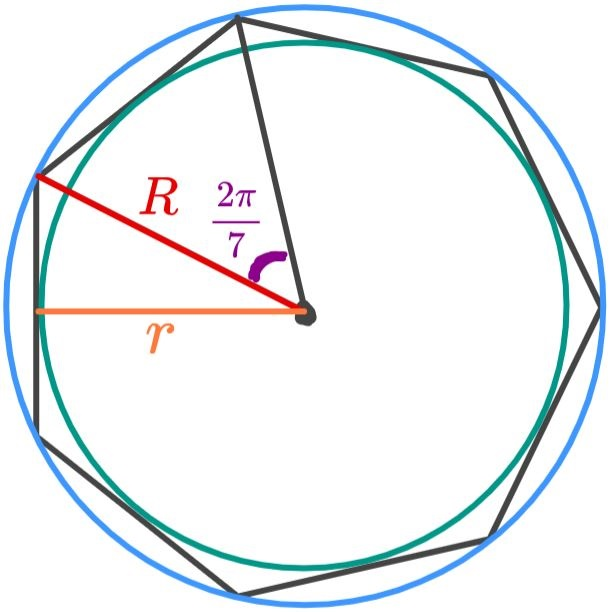
\includegraphics[width=\linewidth]{sol53}\end{figure}\end{minipage}
\end{minipage}}
{Площадь вписанного круга меньше площади описанного круга на $100\sin^2\frac{\pi}{7} \approx 19\%$. Общий случай этой задачи для правильного $n$-угольника даёт следующий результат: $\cos^2\frac{\pi}{n}$ равно отношению площадей кругов, а $\sin^2\frac{\pi}{n}$ равно отношению площадей кольца и большого круга.}{Найти отношение радиусов $\frac rR$.}
\end{problem}

\begin{problem}{Решение кубических уравнений. Формула Кардано, основная теорема алгебры.}{11.1.8}{11D}{*}
{Уравнение 4 степени имеет 4 корня: $x_{00} = 1 - \sqrt{2} - \sqrt{3}$, $x_{10} = 1 + \sqrt{2} - \sqrt{3}$, $x_{01} = 1 - \sqrt{2} + \sqrt{3}$, $x_{11} = 1 + \sqrt{2} + \sqrt{3}$. Объяснить, почему многочлен 4 степени, имеющий такие корни, не может быть разложен в произведение двух квадратных многочленов с рациональными коэффициентами.}
{НаписанноеРешение}
{ВерныйОтвет}{Используй метод неопределённых коэффициентов и проведи мудрый перебор вариантов.}
\end{problem}

\begin{problem}{Решение кубических уравнений. Формула Кардано, основная теорема алгебры.}{11.1.8}{11D}{*}
{Решить уравнение $\,x^4 - 3x^3 - 4x^2 + 5x - 1 = 0$.}
{Быстрая проверка показывает, что если бы данное уравнение имело целый корень, то этот корень являлся бы делителем свободного члена данного многочлена, то есть возможны только два варианта, $x = 1$ и $x = -1$. Однако, оба данных кандидата корнями не являются.\\
Используем идею, что если многочлен имеет рациональные коэффициенты, то его корни сопряжены в $\mathbb{R}$ (то есть, числа $a + b\sqrt{c}$ и $a - b\sqrt{c}$ либо оба являются корнями многочлена, либо оба не являются). Это означает, что многочлен четвёртой степени может либо разложиться в произведение двух квадратных многочленов, либо не разложится совсем. Используем метод неопределённых коэффициентов:\\
$x^4 - 3x^3 - 4x^2 + 5x - 1 = (x^2 + ax + b)(x^2 + cx + d) = 0$. Отсюда получаем \\$\left\{\begin{aligned}
a + c &= -3\\
b + ac + d &= -4\\
ad + bc &= 5\\
bd &= -1.
\end{aligned}\right.\:$ \parbox{13.7cm}{Мы предполагаем, что коэффициенты целые, поэтому получаем, что либо $b = 1$, $d = -1$, либо наоборот, $b = -1$, $d = 1$.\smallskip\\ Однако на самом деле достаточно рассмотреть лишь один из двух вариантов: второй получится перестановкой множителей.}\\
Итак, допустим, что $b = 1$, $d = -1.\,$ Тогда $\,\left\{\begin{aligned}
a + c &= -3\\
ac &= -4\\
c - a &= 5\\
\end{aligned}\right. \;\Leftrightarrow\; \left\{\begin{aligned}
a &= -4\\
c &= 1\\
\end{aligned}\right.$\smallskip\\
Получилось, что $x^4 - 3x^3 - 4x^2 + 5x - 1 = (x^2 - 4x + 1)(x^2 + x - 1) = 0$.\\
Решаем оба квадратных уравнения: $x^2 - 4x + 1 = 0 \;\Rightarrow\; D = 16 - 4 = 12 > 0 \;\Rightarrow\; x_{1,2} = \frac{4 \pm 2\sqrt{3}}{2} = 2 \pm \sqrt{3}$, $x^2 + x - 1 = 0 \;\Rightarrow\; D = 1 + 4 = 5 > 0 \;\Rightarrow\; x_{3,4} = \frac{-1 \pm \sqrt{5}}{2}$.}
{Данное уравнение имеет 4 вещественных корня: $x = 2 \pm \sqrt{3}\,$ и $\,x = \frac{-1 \pm \sqrt{5}}{2}$.}{Что происходит при сопряжении чисел вида $a + b\sqrt{c}$ над $\mathbb{R}$?}
\end{problem}

\begin{problem}{Решение кубических уравнений. Формула Кардано, основная теорема алгебры.}{11.1.8}{11D}{*}
{Решить уравнение $\,x^4 + 3x^3 - x^2 - 4x + 2 = 0$.}
{НаписанноеРешение}
{ВерныйОтвет}{Используй метод неопределённых коэффициентов и проведи мудрый перебор вариантов.}
\end{problem}

\begin{problem}{Решение кубических уравнений. Формула Кардано, основная теорема алгебры.}{11.1.8}{11D red не задача}{(лёгкая)}
{Пробежаться глазами по статье в Википедии про
\textcolor{CornflowerBlue}{\href{https://ru.wikipedia.org/wiki/\%D0\%9A\%D0\%BE\%D0\%BC\%D0\%BF\%D0\%BB\%D0\%B5\%D0\%BA\%D1\%81\%D0\%BD\%D0\%BE\%D0\%B5_\%D1\%87\%D0\%B8\%D1\%81\%D0\%BB\%D0\%BE}{\textit{комплексные числа}}}.\medskip\\ Ознакомиться со статьями о решении уравнений третьей (\textcolor{CornflowerBlue}{\href{https://ru.wikipedia.org/wiki/\%D0\%A4\%D0\%BE\%D1\%80\%D0\%BC\%D1\%83\%D0\%BB\%D0\%B0_\%D0\%9A\%D0\%B0\%D1\%80\%D0\%B4\%D0\%B0\%D0\%BD\%D0\%BE}{\textit{формула Кардано}}}) и четвёртой степеней (\textcolor{CornflowerBlue}{\href{https://ru.wikipedia.org/wiki/\%D0\%9C\%D0\%B5\%D1\%82\%D0\%BE\%D0\%B4_\%D0\%A4\%D0\%B5\%D1\%80\%D1\%80\%D0\%B0\%D1\%80\%D0\%B8}{\textit{формула Феррари}}}).\\
Ознакомиться с утверждением \textcolor{CornflowerBlue}{\href{https://ru.wikipedia.org/wiki/\%D0\%A2\%D0\%B5\%D0\%BE\%D1\%80\%D0\%B5\%D0\%BC\%D0\%B0_\%D0\%90\%D0\%B1\%D0\%B5\%D0\%BB\%D1\%8F_\%D0\%BE_\%D0\%BD\%D0\%B5\%D1\%80\%D0\%B0\%D0\%B7\%D1\%80\%D0\%B5\%D1\%88\%D0\%B8\%D0\%BC\%D0\%BE\%D1\%81\%D1\%82\%D0\%B8_\%D1\%83\%D1\%80\%D0\%B0\%D0\%B2\%D0\%BD\%D0\%B5\%D0\%BD\%D0\%B8\%D0\%B9_\%D0\%B2_\%D1\%80\%D0\%B0\%D0\%B4\%D0\%B8\%D0\%BA\%D0\%B0\%D0\%BB\%D0\%B0\%D1\%85}{\textit{теоремы Абеля-Руффини}}} об отсутствии общей формулы решения в явном виде для уравнений более высоких степеней.}
{НаписанноеРешение}
{ВерныйОтвет}{Подсказка}
\end{problem}

\end{document}